\documentclass[11pt]{article}
\usepackage[margin=1in]{geometry}
\usepackage{amsmath, amssymb}
\usepackage{enumitem}
\usepackage{tikz}
\usepackage{graphicx}
\usepackage{float}
\usepackage{placeins}
\usepackage{booktabs}

\title{HW \#5}
\author{Theo Tarr}
\date{March 5, 2026}

\begin{document}
\maketitle

\section*{1. Reading-Related Question}

\textbf{(a)} The primitive soup hypothesis (Oparin-Haldane) says life began in a dilute ocean where UV light and lightning produced organic compounds like amino acids and nucleotides. A key weakness is specificity: the soup has no way to ensure that polymers form with the correct chemical bonds. Proteins require peptide bonds and RNA requires specific nucleotide linkages, but Miller-type experiments produce a mix of bonds. Wrong linkages block replication entirely.

The primitive pizza hypothesis (Wächtershäuser) says life began on positively charged iron pyrite surfaces. Organic ions bond to the surface and are held in a fixed orientation, able to move only in two dimensions instead of freely in solution. This increases both reaction speed and specificity, and concentrates molecules so they can react. This directly solves the soup's problem because the surface enforces correct orientations for polymerization.

\textbf{(b)} Without replicase enzymes the error rate is very high, too high to replicate any meaningful length of molecule reliably (the error threshold). With replicase but without proofreading, the error rate is $1/1000$ to $1/10{,}000$ per nucleotide. This is because RNA strands separate immediately after copying, so there is no way to check whether each base was paired correctly. Replicase improves accuracy significantly, but without proofreading errors are still too frequent for large genomes, which is expected since enzyme geometry alone improves selectivity but cannot catch all mistakes.

\textbf{(c)} RNA is single-stranded, so there is no complementary strand to use for proofreading. With an error rate of $1/1000$ to $1/10{,}000$ and a human genome of 3 billion bases, every replication cycle would introduce millions of mutations. RNA is also chemically unstable since its $2'$-OH group makes it susceptible to hydrolysis. A human with RNA genes would rapidly accumulate errors that destroy genetic information faster than it can be replicated, making stable complex life impossible.

\section*{2. $^{12}$C--$^{13}$C Fractionation}

\textbf{(a)}

\[
m_\text{proton} = m_\text{neutron} = 1.67 \times 10^{-27} kg
\]
\[
m_{^{12}\text{C}} = 12 \times 1.67\times10^{-27}\ \text{kg} = 2.004\times10^{-26}\ \text{kg}
\]
\[
m_{^{13}\text{C}} = 13 \times 1.67\times10^{-27}\ \text{kg} = 2.171\times10^{-26}\ \text{kg}
\]

\textbf{(b)} Using $E_1 = \frac{h^2}{8mL^2}$ with $L = 2\times10^{-10}\ \text{m}$ and $h = 6.626\times10^{-34}\ \text{J\,s}$:

\[
E_1(^{12}\text{C}) = \frac{(6.626\times10^{-34})^2}{8 \times 2.004\times10^{-26} \times (2\times10^{-10})^2}
= 6.85\times10^{-23}\ \text{J}
= \frac{6.85\times10^{-23}}{1.602\times10^{-19}}\times10^3\ \text{meV} \approx \boxed{0.427\ \text{meV}}
\]
\[
E_1(^{13}\text{C}) = \frac{(6.626\times10^{-34})^2}{8 \times 2.171\times10^{-26} \times (2\times10^{-10})^2}
= 6.32\times10^{-23}\ \text{J}
= \frac{6.32\times10^{-23}}{1.602\times10^{-19}}\times10^3\ \text{meV} \approx \boxed{0.394\ \text{meV}}
\]

Both have the same $n=1$ wave shape (one hump, no internal nodes). Because $^{12}$C is lighter, it has a higher ground-state energy.

\begin{figure}
    \centering
    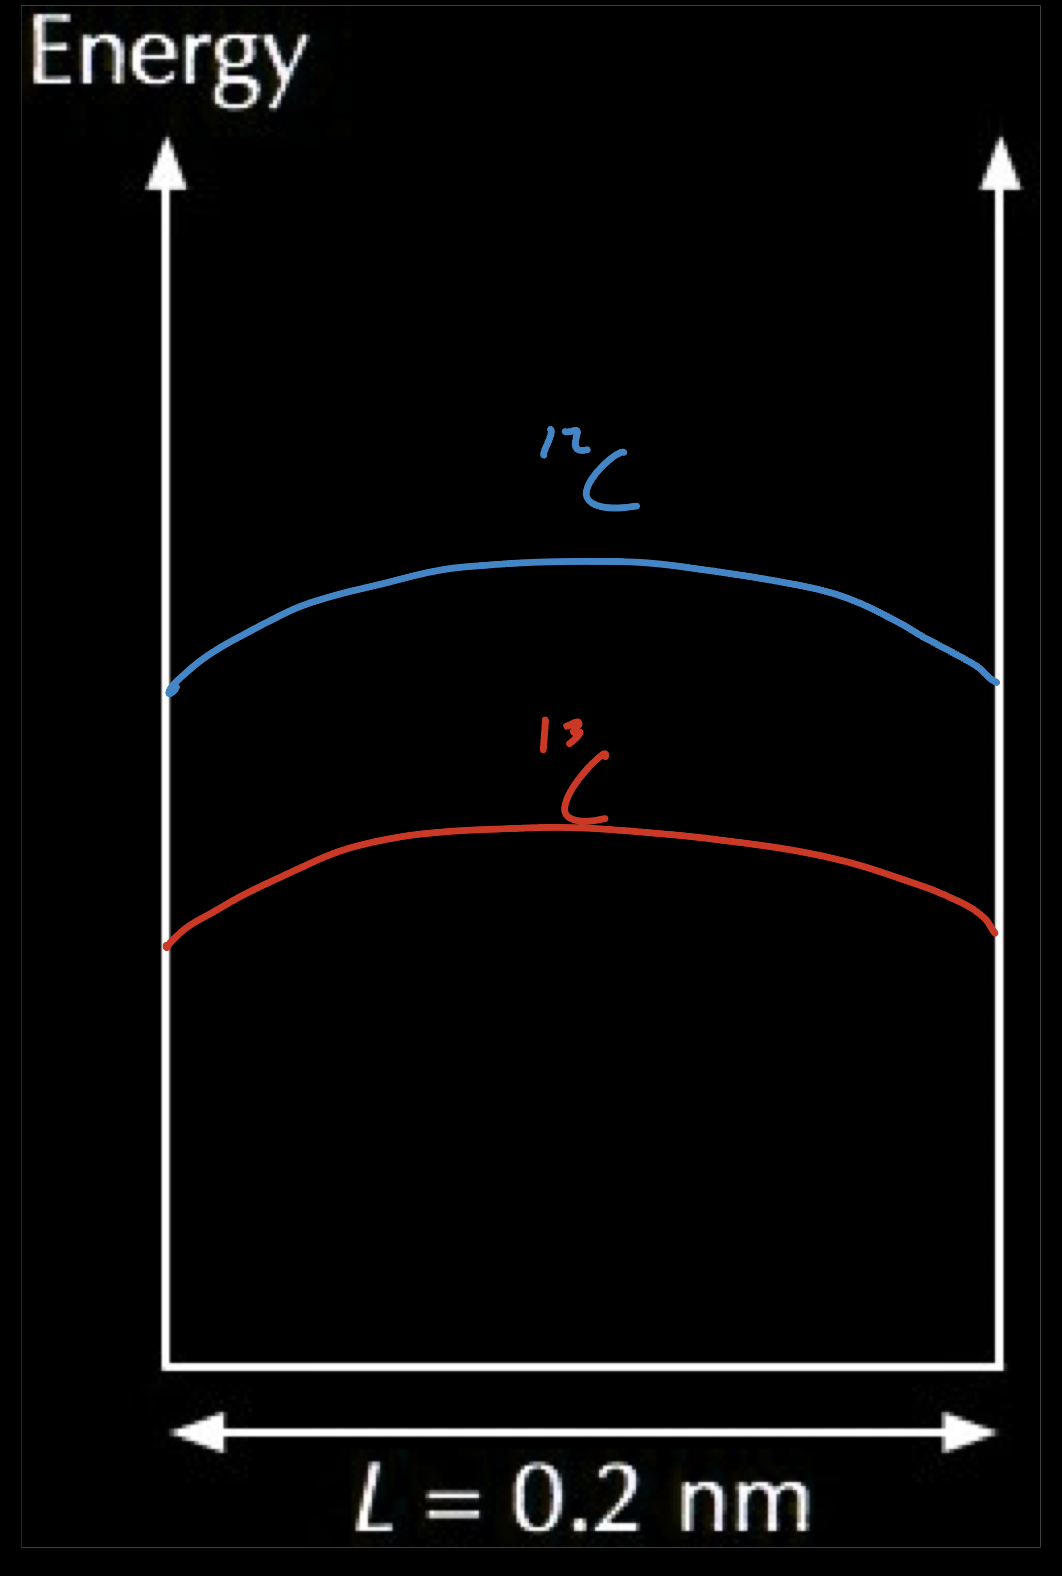
\includegraphics[width=0.5\linewidth]{NBMetadataCache.png}
    \caption{Ground-state ($n=1$) wavefunctions for $^{12}$C (blue) and $^{13}$C (red).}
    \label{fig:placeholder}
\end{figure}

\textbf{(c)} Let $E_\text{ts}$ be the (same) transition-state energy for both isotopes. The activation energy for each is:
\[
E_a = E_\text{ts} - E_1
\]
Since rate $\propto e^{-E_a/k_BT}$, the ratio is:
\[
\frac{\text{rate}(^{12}\text{C})}{\text{rate}(^{13}\text{C})}
= \frac{e^{-(E_\text{ts}-E_1^{12})/k_BT}}{e^{-(E_\text{ts}-E_1^{13})/k_BT}}
= e^{(E_1^{12}-E_1^{13})/k_BT}
\]
\[
\Delta E = E_1(^{12}\text{C}) - E_1(^{13}\text{C}) = 6.85\times10^{-23} - 6.32\times10^{-23} = 5.3\times10^{-24}\ \text{J}
\]
\[
k_BT = (1.381\times10^{-23})(300) = 4.14\times10^{-21}\ \text{J}
\]
\[
\frac{\Delta E}{k_BT} = \frac{5.3\times10^{-24}}{4.14\times10^{-21}} = 1.28\times10^{-3}
\]
\[
\frac{\text{rate}(^{12}\text{C})}{\text{rate}(^{13}\text{C})} = e^{1.28\times10^{-3}} \approx \boxed{1.00128}
\]
$^{12}$C reacts about $0.13\%$ faster than $^{13}$C, consistent with observed isotope fractionation in photosynthesis.

\textbf{(d)} At higher temperature $k_BT$ increases, so $\Delta E/k_BT$ decreases and the rate ratio approaches 1. The fractionation effect weakens and both isotopes react at nearly the same rate.

\textbf{(e)} For $^{13}$C to react faster, the transition state must also have zero-point energy, with $E_\text{ts}(^{12}\text{C}) > E_\text{ts}(^{13}\text{C})$ by more than the ground-state difference. This happens when the bond to carbon is stiffer in the transition state than in the reactant, giving $^{12}$C a larger energy penalty at the transition state so its activation energy ends up higher.

\section*{3. First Cells}

\textbf{(a)} Primitive fatty acid membranes are permeable to nucleotides, so they can cross in and out freely. Inside the vesicle, RNA replication consumes free nucleotides by incorporating them into long polymers that cannot leave. This lowers the internal nucleotide concentration below the outside, creating a gradient that drives more nucleotides in than out.

\textbf{(b)} RNA polymers trapped inside raise the total solute concentration inside the vesicle. Water then flows in by osmosis, trying to equalize the concentration across the membrane, causing the vesicle to swell.

\textbf{(c)} Swollen vesicles have membrane tension, which is lowered when new fatty acids are added to the membrane. This means swollen, RNA-rich vesicles preferentially absorb fatty acids from the surrounding solution and from relaxed, RNA-poor neighbors, which then shrink. Better replicators swell more, steal more membrane, and grow at the expense of poorer replicators -- natural selection at the protocell level.

\textbf{(d)} Szostak proposes temperature cycling driven by volcanic environments. Protocells in a pool near hot rocks would occasionally be carried by convection currents past the rocks, receiving a brief burst of heat that separates the two RNA strands. They then cool rapidly in the bulk cold water, where each single strand acts as a template to form a new complementary strand. This is essentially a natural geothermal version of PCR, requiring no molecular machinery.

\section*{4. Handedness}

\textbf{(a)} Using the Boltzmann distribution for $\Delta E = 10^{-17}\ \text{eV}$:
\[
\frac{P(L)}{P(D)} = e^{\Delta E / k_BT}
\]
\[
k_BT = (8.617\times10^{-5}\ \text{eV/K})(295\ \text{K}) = 0.02542\ \text{eV}
\]
\[
\frac{\Delta E}{k_BT} = \frac{10^{-17}}{0.02542} = 3.93\times10^{-16}
\]
\[
\frac{P(L)}{P(D)} = e^{3.93\times10^{-16}} \approx 1 + 3.93\times10^{-16} \approx \boxed{1.000\,000\,000\,000\,000\,4}
\]
Both forms are essentially equally probable at room temperature.


\textbf{(b)} We want $P(D)/P(L) = 0.1$, so $P(L)/P(D) = 10$:
\[
e^{\Delta E / k_BT} = 10
\]
\[
k_BT = \frac{\Delta E}{\ln 10} = \frac{10^{-17}\ \text{eV}}{2.303} = 4.34\times10^{-18}\ \text{eV}
\]
\[
T = \frac{4.34\times10^{-18}\ \text{eV}}{8.617\times10^{-5}\ \text{eV/K}} \approx \boxed{5.04\times10^{-14}\ \text{K}}
\]

\textbf{(c)} No. The effect at room temperature is only on the order $ 10^{-16}$, which is nowhere near enough to explain how there is near 100\% L-amino acid homochirality in biology.

\textbf{(d)} Logan's alternative explanation is that homochirality was a historical accident. Abiotic chemistry produces a 50/50 mix of L and D amino acids, but by chance one form ended up slightly more prevalent early in the origin of life. Once one handedness had a small advantage, it became locked in and amplified over time since mixing L and D disrupts protein function, making a pure-handedness system strongly favored once it gets started.

\end{document}
